\documentclass[a4paper]{article}
\addtolength{\hoffset}
{-2.25cm}
\addtolength{\textwidth}
{5cm}
\addtolength{\voffset}
{-3.25cm}
\addtolength{\textheight}
{5.5cm}
\setlength{\parskip}{0pt}
\setlength{\parindent}{0in}

\usepackage[utf8]{inputenc}
\usepackage{microtype}
\usepackage[english]{babel}
\usepackage{fancyhdr}
\usepackage{advdate}
\usepackage{enumitem}
\usepackage{amsmath, amssymb}
\usepackage{graphicx}
\usepackage{caption}
\usepackage{subcaption}
\usepackage{float}
\usepackage{titlesec}
\usepackage{wasysym}
\usepackage{url}
\usepackage{hyperref}
\usepackage{tikz, verbatimbox}
\usepackage{fixltx2e}
\usepackage{centernot}
\usepackage{algorithm}
\usepackage{algpseudocode}
\usetikzlibrary{shapes.geometric, arrows}
\usetikzlibrary{positioning}
\usepackage[table]{xcolor}

\graphicspath{{./static/}}
\tikzset{every picture/.style={line width=0.75pt}} %set default line width to 0.75pt

\newcommand{\LComment}[1]{\State \(\triangleright\) \text{#1}}
\MakeRobust{\Call}
\usepackage{pdfpages}
\usetikzlibrary{positioning}

\begin{document}

\fancyhead[c]{}
\hrule \medskip
\begin{minipage}{0.295\textwidth}
\raggedright
Rishabh Indoria\\
21F3001823
\end{minipage}
\begin{minipage}{0.4\textwidth}
\centering
\LARGE
Software Testing
\end{minipage}
\begin{minipage}{0.295\textwidth}
\raggedleft
\today \hfill \\
\end{minipage}
\medskip \hrule
\bigskip

\section{Introduction}
\subsection{Motivation}
\begin{itemize}
    \item \textbf{Introduction to Software Testing} by Paul Ammann and Jeff Offutt, \textbf{The Art of Software Testing} by Glenford J. Myers, \textbf{Software Testing: A Craftsman's Approach} by Paul C. Jorgensen, \textbf{Agile Testing: A practical guide for Testers and Agile Teams} by Lisa Crispin and Janet Gregory.
    \item Software is ubiquitous; Such software should be of very high quality, offer good performance in terms of response time, performance and also have no errors.
    \item It is no longer feasible to shut down a malfunctioning system in order to restore safety.
    \item Errors in software can cost lives, huge financial losses, or simply a lot of irritation.
    \item Testing is the \textbf{predominantly used} technique to find and eliminate errors in software.
\end{itemize}
\subsection{Software Development Life Cycle}
\begin{itemize}
    \item \textbf{SDLC}: term used by the software industry to define a process for designing, developing, testing and maintaining a high quality software product.
    \item The goal is to use SDLC defined processes to develop a high quality software product that meets customer demands.
    \item \textbf{Planning}: Includes clearly identifying customer and/or market needs, pursuing a feasibility study and arriving at an initial set of requirements.
    \item \textbf{Requirements definition}: Includes documenting detailed requirements of various kinds: System-level, functional, software, hardware, quality requirements etc. They get approved by appropriate stakeholders.
    \item \textbf{Requirements analysis}: Includes checking and analyzing requirements to ensure that they are consistent, complete and match the feasibility study and market needs.
    \item \textbf{Design}: Identifies all the modules of the software product, details out the internals of each module, the implementation details and a skeleton of the testing details.
    \item \textbf{Architecture}: Defines the modules, their connections and other dependencies, the hardware, database and its access etc.
    \item \textbf{Development}: The design documents, especially that of low-level design, is used to implement the product. There are usually coding guidelines to be followed by the developers. Extensive unit testing and debugging are also done, usually by the developers. Tracking is done by project management team.
    \item \textbf{Testing}: Involves testing only where the product is thoroughly tested, defects are reported, fixed and re-tested, until all the functional and quality requirements are met.
    \item \textbf{Maintenance}: Done post deployment of product. Add new features as desired by the customer/market. Fix errors, if any, in the software product. Test cases from earlier phases are re-used here, based on need.
    \item \textbf{V-model}: It is a model that focuses on verification and validation. Follows the traditional SDLC life-cycle: Requirements, Design, Implementation, Testing, Maintenance.
    \item \textbf{Agile model}: Agile methodologies are adaptive and focus on fast delivery of features of a software product. All the SDLC steps are repeated in incremental iterations to deliver a set of features. Extensive customer interactions, quick delivery and rapid response to change in requirements.
    \item \textbf{Other Activities}: Project management, includes team management. Project documentation(Traceability matrix is a document that links each artifacts of development phase to those of other phases). Quality Inspection.
    \begin{figure}[H]
        \centering
        \begin{subfigure}[b]{0.45\textwidth}
            \includegraphics[width=\textwidth]{Degree/static/ST_v_model.png}
            \caption{V-Model}
            \label{fig:ST-v-model}
        \end{subfigure}
        \hfill
        \begin{subfigure}[b]{0.45\textwidth}
            \includegraphics[width=\textwidth]{Degree/static/ST_agile_model.png}
            \caption{Agile Model}
            \label{fig:ST-agile-model}
        \end{subfigure}
        \caption{Model Visualization}
        \label{fig:ST-model-visualizations}
    \end{figure}
\end{itemize}
\subsection{Testing Terminologies}
\begin{itemize}
    \item \textbf{Validation}: The process of evaluating software at the end of software development to ensure compliance with intended usage. i.e., checking if the software meets its requirements.
    \item \textbf{Verification}: The process of determining whether the products of a given phase of the software development process fulfill the requirements established at the start of that phase.
    \item \textbf{Fault}: A static defect in the software. It could be a missing function or a wrong function in code.
    \item \textbf{Failure}: An external, incorrect behavior with respect to the requirements or other description of the expected behavior. A failure is a manifestation of a fault when software is executed.
    \item \textbf{Error}: An incorrect internal state that is the manifestation of some fault.
    \item \textbf{Test case}: A test case typically involves inputs to the software and expected outputs. A failed test case indicates an error. A test case also contains other parameters like test case ID, traceability details etc.
    \item \textbf{Unit Testing}: Done by developer during coding.
    \item \textbf{Integration Testing}: Various components are put together and tested. Components could be only software or software and hardware components.
    \item \textbf{System Testing}: Done with full system implementation and the platform on which the system will be running.
    \item \textbf{Acceptance Testing}: Done by end customer to ensure that the delivered products meet the committed requirements.
    \item \textbf{Beta Testing}: Done in a (so-called) beta version of the software by end users, after release.
    \item \textbf{Functional Testing}: Done to ensure that the software meets its specified functionality.
    \item \textbf{Stress Testing}: Done to evaluate how the system behaves under peak/unfavorable conditions.
    \item \textbf{Performance Testing}: Done to ensure the speed and response time of the system.
    \item \textbf{Usability Testing}: Done to evaluate the user interface, aesthetics.
    \item \textbf{Regression Testing}: Done after modifying/upgrading a component, to ensure that the modification is working correctly, and other components are not damaged by the modification.
    \item \textbf{Black-Box Testing}: A method of testing that examines the functionalities of a software/system without looking into its internal design or code.
    \item \textbf{White-Box Testing}: A method of testing that test the internal structure of the design or code of a software.
    \item \textbf{Test Design}: Most critical job in testing. Need to design effective test cases. Apart from specifying the inputs, this involves defining the expected outputs too. Typically, cannot be automated.
    \item \textbf{Test Automation}: Involves converting the test cases into executable scripts. Need to specify how to reach deep parts of the code using just inputs, Observability and Controllability.
    \item \textbf{Test Execution}: Involves running the test on the software and recording the results. Can be fully automated.
    \item \textbf{Test Evaluation}: Involves evaluating the results of testing, reporting identified errors. A difficult problem is to isolate faults, especially in large software and during integration testing.
    \item \textbf{Testing goals}: Organizations tend to work with one or more of the following levels\\
    \textbf{Level 0}: There is no difference between testing and debugging.\\
    \textbf{Level 1}: The purpose of testing is to show correctness.\\
    \textbf{Level 2}: The purpose of testing is to show that software doesn't work.\\
    \textbf{Level 3}: The purpose of testing is not to prove anything specific, but to reduce the risk of using the software.\\
    \textbf{Level 4}: Testing is a mental discipline that helps all IT professionals develop higher quality software.
    \item \textbf{Controllability}: Controllability is about how easy it is to provide inputs to the software module under test, in terms of reaching the module and running the test cases on the module under test.
    \item \textbf{Observability}: Observability is about how easy it is to observe the software module under test and check if the module behaves as expected.
\end{itemize}

\section{Graphs}
\subsection{Basics}
\begin{itemize}
    \item A graph is a tuple $G=(V,E)$ where $V$ is a set of \textbf{nodes/vertices}, and $E\subseteq(V\times V)$ is a set of \textbf{edges}.
    \item Graphs can be \textbf{directed} or \textbf{undirected}.
    \begin{figure}[H]
        \centering
        \begin{subfigure}[b]{0.45\textwidth}
            \centering
            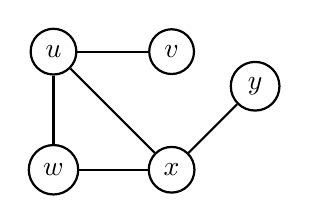
\begin{tikzpicture}[node distance={15mm}, thick, main/.style = {draw, circle}]
                \node[main] (1) {$u$};
                \node[main] (2) [right of=1] {$v$};
                \node[main] (3) [below of=1] {$w$};
                \node[main] (4) [right of=3] {$x$};
                \node[main] (5) [above right of=4] {$y$};

                \draw (1) -- (2);
                \draw (1) -- (3);
                \draw (1) -- (4);
                \draw (3) -- (4);
                \draw (4) -- (5);
            \end{tikzpicture} 
            \caption{A simple undirected graph}
        \end{subfigure}
        \hfill
        \begin{subfigure}[b]{0.45\textwidth}
            \centering
            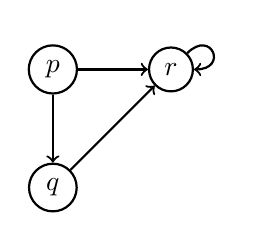
\begin{tikzpicture}[node distance={15mm}, thick, main/.style = {draw, circle}]
                \node[main] (1) {$p$};
                \node[main] (2) [right of=1] {$r$};
                \node[main] (3) [below of=1] {$q$};

                \draw[->] (1) -- (2);
                \draw[->] (1) -- (3);
                \draw[->] (3) -- (2);
                \draw[->] (2) to [out=45,in=0,looseness=5] (2);
            \end{tikzpicture} 
            \caption{A directed graph}
        \end{subfigure}
    \end{figure}
    \item Graphs can finite or infinite.
    \item The \textbf{degree} of a vertex is the number of edges that are connected to it. Edges connected to a vertex are said to be \textbf{incident} on the vertex.
    \item There are designated special vertices like \textbf{initial} and \textbf{final} vertices. These vertices indicate beginning and end of a property that the graph is modeling.
    \item Typically, there is only one initial vertex, but there could be several final vertices.
    \begin{figure}[H]
        \centering
        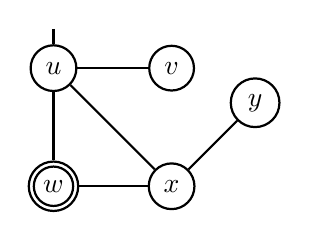
\begin{tikzpicture}[node distance={15mm}, thick, main/.style = {draw, circle}]
            \node[main] (1) {$u$};
            \node[main] (2) [right of=1] {$v$};
            \node[main] (3) [below of=1] {$w$};
            \node[main, minimum size=0.5cm] (33) [below of=1] {};
            \node[main] (4) [right of=3] {$x$};
            \node[main] (5) [above right of=4] {$y$};

            \draw (0,0.5) -- (1);
            \draw (1) -- (2);
            \draw (1) -- (3);
            \draw (1) -- (4);
            \draw (3) -- (4);
            \draw (4) -- (5);
        \end{tikzpicture}
        \caption{Graph with initial and final vertices}
    \end{figure}
    \item Most of these graphs will have \textbf{labels} associated with vertices and edges. Labels or annotations could be details about the artifact that the graphs are modelling. Tests are intended to cover the graph in some way.
    \begin{figure}[H]
        \centering
        \begin{subfigure}[b]{0.45\textwidth}
            \begin{verbatim}
                if(x<y){
                y = 0;
                x = x+1;
                }else{
                x = y+1;
                }
                z = x+1;
            \end{verbatim}
            \caption{A sample code}
        \end{subfigure}
        \hfill
        \begin{subfigure}[b]{0.45\textwidth}
            \begin{myverbbox}{\edgeONE}
                x>=y
            \end{myverbbox}
            \begin{myverbbox}{\edgeTWO}
                x<y
            \end{myverbbox}
            \begin{myverbbox}{\vertexONE}
                x = y+1
            \end{myverbbox}
            \begin{myverbbox}{\vertexTWO}
                y = 0
                x = x+1
            \end{myverbbox}
            \begin{myverbbox}{\vertexTHREE}
                z = x+1
            \end{myverbbox}
            \hspace{-2cm}
            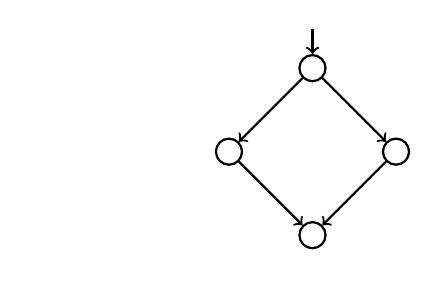
\begin{tikzpicture}[node distance={15mm}, thick, main/.style = {draw, circle}]
                \node[main] (1) {};
                \node[main] (2) [below right of=1] {};
                \node at (0.5, -1.3) {\vertexONE};
                \node[main] (3) [below left of=1] {};
                \node at (-3.5, -1.3) {\vertexTWO};
                \node[main] (4) [below left of=2] {};
                \node at (-0.5, -2.3) {\vertexTHREE};
                \node at (-0.5,-0.5) {\edgeONE};
                \node at (-2.5, -0.5) {\edgeTWO};

                \draw[->] (0,0.5) -- (1);
                \draw[->] (1) -- (2);
                \draw[->] (1) -- (3);
                \draw[->] (2) -- (4);
                \draw[->] (3) -- (4);
            \end{tikzpicture}
            \caption{A Control Flow Graph}
        \end{subfigure}
        \caption{Example of a CFG}
    \end{figure}
    \item A \textbf{path} is a sequence of vertices $v_1,v_2,...,v_n$ such that $(v_i,v_{i+1})\in E$.
    \item \textbf{Length} of a path is the number of edges that occur in it. A single vertex path has length 0.
    \item \textbf{Sub-path} of a path is a sub-sequence of vertices that occur in the path.
    \item A vertex $v$ is \textbf{reachable} from some other vertex if there is a path connecting them.
    \item An edge $e=(u,v)$ is \textbf{reachable} if there is a path that goes to vertex $u$ and then goes to vertex $v$.
    \item A \textbf{test path} is a path that starts in an initial vertex and ends in a final vertex. These represent execution of test cases.
    \item Some test paths can be executed by many test cases: \textbf{Feasible paths}.
    \item Some test paths cannot be executed by any test case: \textbf{Infeasible paths}.
    \item A test path $p$ \textbf{visits} a vertex $v$ if $v$ occurs in path $p$. A test path $p$ \textbf{visits} an edge $e$ if $e$ occurs in the path $p$.
    \item A test path $p$ \textbf{tours} a path $q$ if $q$ is a sub-path of $p$.
    \item When a test case $t$ executes a path, we call it the \textbf{test path} executed by $t$, denoted by $path(t)$.
    \item The set of test paths executed by a set of test cases $T$ is denoted by $path(T)$.
    \item \textbf{Test requirement} describes properties of test paths.
    \item \textbf{Test Criterion} are rules that define test requirements.
    \item \textbf{Satisfaction}: Given a set $TR$ of test requirements for a criterion $C$, a set of tests $T$ satisfies $C$ on a graph iff for every test requirement in $t\in TR$, there is a test path in $path(T)$ that meets the test requirement $t$.
    \item \textbf{Structural Coverage Criteria}: Defined on a graph just in terms of vertices and edges.
    \item \textbf{Data Flow Coverage Criteria}: Requires a graph to be annotated with references to variables and defines criteria requirements based on the annotations.
\end{itemize}

\subsection{Elementary Graph Algorithms}
\begin{itemize}
    \item Two standard ways of representing graphs: \textbf{adjacency matrix} or \textbf{adjacency lists}.
    \item Adjacency list representation provides a compact way to represent \textbf{sparse} graphs, i.e., graphs for which $|E|$ is much less than $|V|^2$. For each $u\in V$, $Adj[u]$ contains all vertices $v$ such that $(u,v)\in E$, i.e., it contains all edges incident with $u$. Represented in $\Theta(|V|+|E|)$ memory.
    \item Adjacency matrix representation provides a compact way to represent \textbf{dense} graphs, i.e., graphs for which $|E|$ is close to $|V|^2$. This is a $|V|\times |V|$ matrix, where $a_{ij}=1$ if there is an edge going from $i$ to $j$.
    \item \textbf{Breadth First Search}: Computes the "distance" from $s$ to each reachable vertex.
    \begin{algorithm}[H]
        \caption{Breadth First Search}\label{alg:ST-BFS}
        \begin{algorithmic}[1]
            \Statex \Call{BFS}{$G$}
            \For{each vertex $u\in G,V-\{s\}$}
                \State $u.color$ = $WHITE$, $u.d=\infty$, $u.\pi$ = NIL
            \EndFor
            \State $s.color$ = $BLUE$, $s.d=0$, $s.\pi$ = NIL
            \State $Q$ = $\phi$
            \State \Call{Enqueue}{$Q,s$}
            \While{$Q\neq \phi$}
                \State $u$ = \Call{Dequeue}{$Q$}
                \For{each $v\in G.Adj[u]$}
                    \If{$v.color$ == $WHITE$}
                        \State $v.color$ = $BLUE$
                        \State $v.d$ = $u.d$ + 1
                        \State $v.\pi$ = $u$
                        \State \Call{Enqueue}{$Q,v$}
                    \EndIf
                \EndFor
                \State $u.color$ = $BLACK$
            \EndWhile
        \end{algorithmic}
    \end{algorithm}
    \item \textbf{Depth First Search}
    \begin{algorithm}[H]
        \caption{Depth First Search}
        \begin{algorithmic}[1]
            \Statex \Call{DFS}{$G$}
            \For{each vertex $u\in G.V$}
                \State $u.color$ = $WHITE$
                \State $u.\pi$ = $NIL$
            \EndFor
            \State $time$ = 0
            \For{each vertex $u\in G.V$}
                \If{$u.color$ == $WHITE$}
                    \State \Call{DFS-Visit}{$G,u$}
                \EndIf
            \EndFor
            \Statex
            \Statex \Call{DFS-Visit}{$G,u$}
            \State $time$ = $time+1$
            \State $u.d$ = $time$
            \State $u.color$ = $GRAY$
            \For{each $v\in G.Adj[u]$}
                \If{$v.color$ == $WHITE$}
                    \State $v.\pi$ = $u$
                    \State \Call{DFS-Visit}{$G,v$}
                \EndIf
            \EndFor
            \State $u.color$ = $BLACK$
            \State $time$ = $time+1$
            \State $u.f$ = $time$
        \end{algorithmic}
    \end{algorithm}
\end{itemize}

\subsection{Structural Graph Coverage}
\begin{itemize}
    \item \textbf{Node Coverage} requires that the test cases visit each node in the graph once. Test set $T$ satisfies node coverage on graph $G$ iff for every syntactically reachable node $n\in G$, there is some path $p$ in $path(T)$ such that $p$ visits $n$.
    \item \textbf{Edge Coverage}: $TR$ contains each reachable path of length up to $1$, inclusive, in $G$. Edge coverage is slightly stronger than node coverage. Allowing length up to 1 allows edge coverage to subsume node coverage.
    \item \textbf{Edge-Pair Coverage}: $TR$ contains each reachable path of length up to 2, inclusive in $G$. Paths of length up to 2 correspond to pairs of edges.
    \item \textbf{Complete path coverage}: $TR$ contains all paths in $G$. Unfortunately, this can be an infeasible test requirement, due to loops.
    \item \textbf{Specified path coverage}: $TR$ contains a set $S$ of paths, where $S$ is specified by the user/tester.
    \item A path from $n_i$ to $n_j$ is \textbf{simple} if no node appears more than once, except possible the first and last node.
    \item A \textbf{prime path} is a simple path that does not appear as a proper sub-path of any other simple path.
    \item \textbf{Prime path coverage}: $TR$ contains each prime path in $G$. Ensures that loops are skipped as well as executed. It subsumes node and edge coverage.
    \item \textbf{Tour with side trips}: A test path $p$ tours a sub-path $q$ with side trips iff every edge $q$ is also in $p$ in the same order. the tour can include a side trip, as long as it comes back to the same node.
    \item \textbf{Tours with detours}: A test path $p$ tours a sub-path $q$ with detours iff every node in $q$ is also in $p$ in the same order. The tour can include a detour from node $n$ as long as it comes back to the prime path at a successor of $n$.
    \item \textbf{Best Effort Touring}: Satisfy as many test requirements as possible without sidetrips. Allow sidetrips to try to satisfy remaining test requirements.
    \item \textbf{Round trip path}: A prime path that starts and ends at the same node.
    \item \textbf{Simple round trip coverage}: $TR$ contains at least one round trip path for each reachable node in $G$ that begins and ends in a round trip path.
    \item \textbf{Complete round trip coverage}: $TR$ contains all round trip paths for each reachable node in $G$.
    \begin{figure}[H]
        \centering
        \includegraphics[width=0.5\linewidth]{Degree//static/ST_Structural_Coverage.png}
        \caption{Structure Coverage Criteria Subsumption}
        \label{fig:ST-structure-coverage}
    \end{figure}
\end{itemize}

\subsection{Algorithms: Structural Graph Coverage Criteria}
\begin{itemize}
    \item There are two entities related to coverage criteria: Test requirement, and Test case as a test path, if the test requirement is feasible.
    \item Test requirements for node and edge coverage are already given as a part of the graph modeling the software artifact. Test paths to achieve node and edge coverage can be obtained by simple modifications to BFS.
    \item $TR$ for edge-pair coverage is all paths of length two in a given graph. Need to include paths that involve self-loops too.
    \begin{algorithm}[H]
        \caption{Simple Edge-Pair Algorithm}
        \begin{algorithmic}[1]
            \For{each node $u$ in the graph}
                \For{each node $v$ in $Adj[u]$}
                    \For{each node $w$ in $Adj[v]$}
                        \State Output path $u--v--w$
                    \EndFor
                \EndFor
            \EndFor
        \end{algorithmic}
    \end{algorithm}
    \item Prime Path Algorithm
    \begin{algorithm}[H]
        \caption{Computing prime paths}
        \begin{algorithmic}[1]
            \State $Loops$ = [ ]
            \State $Terminate$ = [ ]
            \State $Q$ = $\phi$
            \For{each $v\in G$}
                \State \Call{Enqueue}{$Q,[v]$}
            \EndFor
            \While{$Q\neq \phi$}
                \State $path$ = \Call{Dequeue}{$Q$}
                \For{each $v\in G.Adj[path[-1]]$}
                    \If{$v$ is a final vertice}
                        \State $Terminate$ = $Terminate$ ++ ($path$ ++ $v$)
                    \ElsIf{$v$ in $path$ and $v$ == $path[0]$}
                        \State $Loops$ = $Loops$ ++ ($path$ ++ $v$)
                    \ElsIf{$v$ in $path$}
                        \State continue
                    \Else
                        \State \Call{Enqueue}{$Q, path$ ++ $v$}
                    \EndIf
                \EndFor
            \EndWhile
            \State \Return $Loops$, $Terminate$
        \end{algorithmic}
    \end{algorithm}
    \item To enumerate test paths for prime path coverage: Start with the longest prime paths and extend each of them to the initial and the final nodes in the graph.
\end{itemize}

\subsection{Control Flow Graphs for Code}
\begin{itemize}
    \item Modelling control flow in code as graphs. Using structural coverage criteria to test control flow in code.
    \item Typically used to test a particular function or procedure or a method.
    \item A \textbf{Control Floe Graph} models all executions of a method by describing control structures.
    \item \textbf{Nodes}: Statements or sequences of statements (basic blocks).
    \item \textbf{Basic Block}: A sequence of statements such that if the first statement is executed, all statements will be (no branches).
    \item \textbf{Edges}: Transfer of control from one statement to the next.
    \item CFGs are often annotated with extra information to model data, this includes branch predicates, Definitions and/or uses.
    \begin{figure}[H]
        \centering
        \begin{subfigure}[b]{0.45\textwidth}
            \begin{verbatim}
                x = 0;
                while(x<y){
                    y = f(x,y);
                    if(y == 0){
                        break;
                    }else if(y<0){
                        y = y*2;
                        continue;
                    }
                    x = x+1;
                }
                print(y);
            \end{verbatim}
            \caption{While loop with break and continue}
        \end{subfigure}
        \hfill
        \begin{subfigure}[b]{0.45\textwidth}
            \begin{myverbbox}{\vertexONE}
                x = 0;
            \end{myverbbox}
            \begin{myverbbox}{\edgeONE}
                x<y;
            \end{myverbbox}
            \begin{myverbbox}{\edgeTWO}
                x>=y;
            \end{myverbbox}
            \begin{myverbbox}{\vertexTWO}
                y = f(x,y);
            \end{myverbbox}
            \begin{myverbbox}{\edgeTHREE}
                y == 0;
            \end{myverbbox}
            \begin{myverbbox}{\edgeFOUR}
                y<0;
            \end{myverbbox}
            \begin{myverbbox}{\edgeFIVE}
                y>0;
            \end{myverbbox}
            \begin{myverbbox}{\vertexTHREE}
                x = x+1;
            \end{myverbbox}
            \begin{myverbbox}{\vertexFOUR}
                print(y);
            \end{myverbbox}
            \begin{myverbbox}{\vertexFIVE}
                break;
            \end{myverbbox}
            \begin{myverbbox}{\vertexSIX}
                y = y*2;
                continue;
            \end{myverbbox}
            \hspace{-2.5cm}
            \begin{tikzpicture}[node distance={15mm}, thick, main/.style = {draw, circle}]
                \node[main] (1) {1};
                \node at (-0.5, 0) {\vertexONE};
                \node[main] (2) [below of=1] {2};
                \node at (-2.2, -2.05) {\edgeONE};
                \node at (-0.3, -2.05) {\edgeTWO};
                \node[main] (3) [below right of=2] {7};
                \node at (0.8, -2.6) {\vertexFOUR};
                \node[main, minimum size=0.5cm] (33) [below right of=2] {};
                \node[main] (4) [below left of=2] {3};
                \node at (-4, -2.6) {\vertexTWO};
                \node at (-1.5, -3) {\edgeTHREE};
                \node at (-2.2, -3.6) {\edgeFOUR};
                \node at (-3.2, -3.1) {\edgeFIVE};
                \node[main] (5) [below left of=4] {5};
                \node at (-5, -3.7) {\vertexSIX};
                \node[main] (6) [below right of=4] {4};
                \node at (-0.5, -4) {\vertexFIVE};
                \node[main] (7) [below of=4] {6};
                \node at (-2, -4.8) {\vertexTHREE};
                \node[main] (8) [below left of=5] {2};

                \draw[->] (0,0.5) -- (1);
                \draw[->] (1) -- (2);
                \draw[->] (2) -- (3);
                \draw[->] (2) -- (4);
                \draw[->] (4) -- (5);
                \draw[->] (4) -- (6);
                \draw[->] (4) -- (7);
                \draw[->] (6) -- (3);
                \draw[->] (5) -- (8);
                \draw[->] (7) -- (8);
            \end{tikzpicture}
            \caption{A Control Flow Graph}
        \end{subfigure}
        \caption{Example of a CFG}
    \end{figure}
\end{itemize}

\subsection{Data Flow in Graphs}
\begin{itemize}
    \item Graph models of programs can be tested adequately by including values of variables(data values) as a part of the model.
    \item Data values are created at some point in the program and use later. They can be used several times.
    \item A \textbf{definition (def)} is a location where a value of a variable is stored into memory.
    \item A \textbf{use} is a location where a value of a variable is accessed.
    \item As a program executes, data values are carried from their defs to uses. We call these du-pairs or def-use pairs.
    \item A \textbf{du-pair} is a pair of location ($l_i,l_j$) such that a variable $v$ is defined at $l_i$ and used at $l_j$.
    \item Let $V$ be the set of variables that are associated with the program artifact being modelled as a graph.\\
    The subset of $V$ that each node $n$ (edge $e$) defines is called $def(n)(def(e))$.\\
    The subset of $V$ that each node $n$ (edge $e$) uses is called $use(n)(use(e))$.
    \item A def of a variable may or may not reach a particular use.
    \item A path from $l_i$ to $l_j$ is \textbf{def-clear} with respect to variable $v$ if $v$ is not given another value on any of the nodes or edges in the path.
    \item If there is a def-clear path from $l_i$ to $l_j$ with respect to $v$, the def of $v$ at $l_i$ \textbf{reaches} the use at $l_j$.
    \item A \textbf{du-path} with respect to a variable $v$ is a simple path that is def-clear from a def of $v$ to a use of $v$.
    \item $du(n_i,n_j,v)$: The set of du-paths from $n_i$ to $n_j$ for variable $v$.
    \item $du(n_i,v)$: The set of du-paths that start at $n_i$ for variable $v$.
    \item In testing literature, there are two notions of uses available.\\
    If $v$ is used in a computational or output statement, the use is referred to as \textbf{computation use} (or \textbf{c-use}).\\
    If $v$ is used in a conditional statement, its use is called as \textbf{predicate use} (or \textbf{p-use}).
    \item Data flow coverage criteria will be defined as sets of du-paths. Such du-paths will be grouped to define the data flow coverage criteria.
    \item The \textbf{def-path set} $du(n_i,v)$ is the set of du-paths with respect to variable $v$ that start at node $n_i$.
    \item A \textbf{def-pair set}, $du(n_i,n_j,v)$ is the set of du-paths with respect to variable $v$ that start at node $n_i$ and end at node $n_j$.
    \item It can be clearly seen that $du(n_i,v)=\bigcup_{n_j}du(n_i,n_j,v)$.
    \item A test path $p$ is said to \textbf{du tour} a sub-path $d$ with respect to $v$ if $p$ tours $d$ and the portion of $p$ to which $d$ corresponds is def-clear with respect to $v$.
    \item We can allow \textbf{def-clear side trips} with respect to $v$ while touring a du-path, if needed.
    \item There are three common data flow criteria
    \begin{enumerate}
        \item TR: Each def reaches at least one use.\label{enum:ST-data-flow-1}
        \item TR: Each def reaches all possible uses.\label{enum:ST-data-flow-2}
        \item TR: Each def reaches all possible uses through all possible du-paths.\label{enum:ST-data-flow-3}
    \end{enumerate}
    \item We assume every use is preceded by a def, every def reaches at least one use, and for every node with multiple out-going edges, at least one variable is used on each out edge, and the same variables are used on each out edge.
    \item\textbf{Subsumption}: \textcircled{\raisebox{-0.9pt}{\ref{enum:ST-data-flow-3}}}$\rightarrow$\textcircled{\raisebox{-0.9pt}{\ref{enum:ST-data-flow-2}}}$\rightarrow$\textcircled{\raisebox{-0.9pt}{\ref{enum:ST-data-flow-1}}}
    \item Prime path coverage subsumes all-du-paths coverage.
\end{itemize}

\section{Integration Testing}
\subsection{Introduction}
\begin{itemize}
    \item Software design basically dictates how the software is organized into \textbf{modules}.
    \item Modules interact with each other using well-defined \textbf{interfaces}.
    \item \textbf{Integration testing} involves testing if the modules that have been put together as per design meet their functionalities and if the interfaces are correct.
    \item Begins after unit testing, each module has been unit tested.
    \item \textbf{Procedure call interface}: A procedure/method in one module calls a procedure/method in another module. Control can be passed in both directions.
    \item \textbf{Shared memory interface}: A block of memory is shared between two modules. Data is written to/read from the memory block by the modules. The memory block itself can be created by a third module.
    \item \textbf{Message-passing interface}: One module prepares a message of a particular type and send it to another module through this interface. Client-server systems and web-based systems use such interfaces.
    \item Empirical studies account for up to quarter of all the errors in a system to be interface errors.
    \item Integration testing need not wait until all the modules of a system are coded and unit tested.
    \item When testing incomplete portions of software, we need extra software components, sometimes called \textbf{scaffolding}.
    \item \textbf{Test stub} is a skeletal or special purpose implementation of a software module, used to develop or test a component that calls the stub or otherwise depends on it.
    \item \textbf{Test driver} is a software component or test tool that replaces a component that tales care of the control and/or the calling of a software component.
    \item There are five approaches to do integration testing: Incremental, Top-down, Bottom-up, Sandwich, and Big Bang.
    \item \textbf{Incremental approach}: Integration testing is conducted in an incremental manner. The complete system is built incrementally, cycle by cycle, until the entire system is operational. Each cycle is tested by integrating the corresponding modules, errors are fixed before the testing of next cycle begins.
    \item \textbf{Top-down approach to integration testing}: Works well for systems with hierarchical design. 
    \item In hierarchical design, there is a first top-level module, which is decomposed into some second-level modules, some of which, are in turn, decomposed into third-level modules and so on. Terminal modules are those that are not decomposed and can occur at any level. Module hierarchy is the reference document.
    \item It could be the case that A and B are ready but C and D are not, so we can develop stubs for C and D for testing interface between A and B. We keep doing this level by level.
    \item \textbf{Bottom-up approach}: Now we basically start with the lowest level modules and write test drivers to test integration.
    \item Basic difference between top-down and bottom-up is that top-down uses only test stubs and bottom-up uses test drivers.
    \item \textbf{Sandwich} approach tests a system by using a mix of top-down and bottom-up testing.
    \item \textbf{Big Bang Approach}: All individually tested modules are put together to construct the entire system which is tested as a whole.
    \begin{figure}[H]
        \centering
        \includegraphics[width=0.3\linewidth]{Degree//static/ST_module_heirarchy.png}
        \caption{Module Hierarchy}
        \label{fig:ST-module-heirarchy}
    \end{figure}
\end{itemize}

\subsection{Design Integration Testing}
\begin{itemize}
    \item Graph models for integration testing are called \textbf{Call graphs}.
    \item For graph models, nodes now become modules/test stubs/test drivers and edges become interfaces.
    \item \textbf{Structural coverage criteria}: Deals with calls over interfaces.
    \item \textbf{Data flow coverage criteria}: Deals with exchange of data over interfaces.
    \item Node coverage will be to call every module at least once.
    \item Edge coverage is to execute every call at least once.
    \item Specified path coverage can be used to test a sequence of method calls.
    \item Data flow interfaces among modules are more complicated than control flow interfaces.
    \item \textbf{Caller}: A module that invokes/calls another module.
    \item \textbf{Callee}: The module that is called.
    \item \textbf{Call site}: The statement or node where the call appears in the code.
    \item \textbf{Actual parameters}: Variables in the caller.
    \item \textbf{Formal parameters}: Variables in the callee.
    \item \textbf{Coupling variables} are variables that are defined in one unit and used in the other.
    \item \textbf{Parameter coupling}: Parameters are passed in calls.
    \item \textbf{Shared data coupling}: Two units access the same data through global or shared variables.
    \item \textbf{External device coupling}: Two units access an external object like a file.
    \item \textbf{Message-passing interfaces}: Two units communicate by sending and/or receiving messages over buffers/channels.
    \item Since focus is on testing interfaces, we consider the \textbf{last definitions} of variables before calls to and returns from the called units and the \textbf{first uses} inside the modules and after calls.
    \item \textbf{Last-def}: The set of nodes that define a variable $x$ and has a def-clear path from the node through a call site to a use in the other module. Can be in either direction.
    \item \textbf{First-use}: The set of nodes that have uses of a variable $y$ and for which there is a def-clear and use-clear path from the call site to the nodes.
    \item A \textbf{coupling du-path} is from a last-def to a first-use.
    \item \textbf{All-coupling-def coverage}: A path is to be executed from every last-def to at least one first-use.
    \item \textbf{All-coupling-use coverage}: A path is to be executed from every last-def to every first-use.
    \item \textbf{All-coupling-Du-paths coverage}: Every simple path from every last-def to every first-use needs to be executed.
    \item The above criteria can be met with side trips.
    \item Only variables that are used or defined in the callee are considered for du-pairs and criteria.
    \item \textbf{Transitive du-pairs} (A calls B, B calls C and there is a variable defined in A and used in C) is not supported in this analysis.
\end{itemize}

\section{Specification Testing}
\subsection{Sequencing Constraints}
\begin{itemize}
    \item A \textbf{design specification} describes aspects of what behavior a software should exhibit. Behaviour exhibited by software need not mean the implementation directly. It could be a \textbf{model} of the implementation.
    \item For testing with graphs, we consider two types of design specifications. \textbf{Sequencing constraints} on methods/functions, and \textbf{State behavior} descriptions of software.
    \item \textbf{Sequencing constraints} are rules that impose constraints on the order in which methods may be called.
    \item Typically encoded as preconditions or other specifications. They may or may not be given as a part of the specification or design.
    \item Consider the example of a simple Queue, a precondition can be that at least one element must be on the queue before removing and a postcondition can be that $e$ is on the end of the queue to enqueue $e$.
    \item Simple sequencing constraint: enqueue must be called before dequeue.
    \item This does not include the requirement that we must have at least as many enqueue calls as dequeue calls. Need \textit{memory} which can be captured in the \textit{state} of the queue as the application code executes.
    \item Absence of sequencing constraints usually indicates more faults.
\end{itemize}

\subsection{Finite State Machines}
\begin{itemize}
    \item A \textbf{Finite State Machine} is a graph that describes how software variables are modified during execution.
    \item Nodes: \textbf{States}, representing sets of values for (key) variables.
    \item Edges: \textbf{Transitions}, which model possible changes from one state to another. Transitions have \textbf{guards} and/or \textbf{actions} associated with them.
    \item FSMs can model many kinds of systems like embedded software, abstract data types, hardware circuits etc.
    \item Creating FSM models for design helps in precise modelling and early detection of errors through analysis of the model.
    \item Many modelling notations support FSMs: Unified Modeling Language(UML), state tables, Boolean logic etc.
    \item FSMs are good for modelling control intensive applications not ideal for modelling data intensive applications.
    \item FSMs can be annotated with different types of \textbf{actions}: Actions on transitions, Entry actions to nodes, Exit actions on nodes.
    \item Actions can express changes to variables or conditions on variables.
    \item \textbf{Preconditions (guards)}: Conditions that must be true for transition to be taken.
    \item \textbf{Triggering events}: Changes to variables that cause transitions to be taken.
    \item Node coverage: Execute every state(state coverage).
    \item Edge coverage: Execute every transition(transition coverage).
    \item Edge-pair coverage: Execute every pair of transitions(transition-pair).
    \item Control flow graphs are \textbf{not} FSMs representing software/codes.
    \item Call graphs are also \textbf{not} FSMs representing software/codes.
    \item We need to consider values of variables to represent states of FSMs and statements/actions that result in change of values of variables(states) result in transitions.
\end{itemize}

\section{Testing Source Code: Classical Coverage Criteria}
\begin{itemize}
    \item The most common graph model for source code is control flow graph.
    \item Structural coverage criteria over control flow graphs deal with \textbf{covering} the code in some way or other.
    \item Data flow graphs augments the control flow with data.
    \item \textbf{Code coverage}: Statement coverage, branch coverage, decision coverage, Modified Condition Decision Coverage(MCDC), path coverage etc.
    \item Node coverage is same as statement coverage, edge coverage is same as branch, and prime path coverage is the same as loop coverage.
    \item \textbf{Cyclomatic complexity}: Basis path testing, structural testing. It is a software metric used to indicate the (structural) complexity of a program.
    \item Cyclomatic complexity represents the number of \textbf{linearly independent paths} in the control flow graph of a program.
    \item \textbf{Basis path testing} deals with testing each linearly independent path in the CFG of the program.
    \item A \textbf{linearly independent path} of execution in the CFG of a program is a path that does not contain other paths within it. This is very similar to prime paths, every linearly independent path is a prime path.
    \item The cyclomatic complexity $M=E-N+2P$, where $E$ is the number of edges, $N$ is the number of nodes, and $P$ is the number of connected components.
    \item When graph correspond to a single program, $M=E-N+2$.
    \item Another way of measuring cyclomatic complexity is to consider \textit{strongly connected components} in CFG. Can be obtained by connecting the final node back to the initial node. Cyclomatic complexity obtained this way is popularly called as \textbf{cyclomatic number}.
    \item If it is less than 10 then the code is not too complex.
    \item \textbf{Data flow testing}: Data flow coverage.
    \item \textbf{Decision-to-decision path} is a path of execution between two decisions in the CFG.
    \item A \textbf{chain} is a path in which initial and terminal vertices are distinct. All the interior vertices have both in-degree and out-degree as 1.
    \item A \textbf{maximal chain} is a chain that is not a part of any other.
    \item A \textbf{DD-path} is a set of vertices in the CFG that satisfies one of the following conditions:
    \begin{enumerate}
        \item It consists of a single vertex with in-degree 0(initial vertex).
        \item It consists of a single vertex with out-degree 0(terminal vertex).
        \item It consists of a single vertex with in-degree $\geq 2$ or out-degree $\geq 2$(decision vertices).
        \item It consists of a single vertex with in-degree and out-degree as 1.
        \item It is a maximal chain of length $\geq 1$.
    \end{enumerate}
    \begin{figure}[H]
        \centering
        \includegraphics[width=0.5\linewidth]{Degree//static/ST_Graph_summary.png}
        \caption{Graph Coverage Criteria Summary}
        \label{fig:ST-graph-coverage-summary}
    \end{figure}
\end{itemize}

\section{Logic}
\subsection{Basics}
\begin{itemize}
    \item The fragment of logic that we consider is popularly known as \textbf{predicate logic} or \textbf{first order logic}.
    \item An \textbf{atomic proposition} is a term that is either \textbf{true} or \textbf{false}.
    \item Propositional logic deals with combining propositions using \textbf{logical connectives} to form \textbf{formulas} which are complicated statements.
    \item Common logical connectives used in proportional logic are
    \begin{enumerate}
        \item $\lor$ Disjunction
        \item $\land$ conjunction
        \item $\neg$ negation
        \item $\supset$ or $\implies$ implies
        \item $\equiv$ or $\iff$ equivalence
    \end{enumerate}
    \item The set $\phi$ of formulas of propositional logic is the smallest set satisfying the following conditions
    \begin{enumerate}
        \item All atomic propositions is a member of $\phi$
        \item If $\alpha$ is a member of $\phi$, so is $\neg \alpha$
        \item If $\alpha$ and $\beta$ are members of $\phi$ so is $\alpha \lor \beta$
    \end{enumerate}
    \item Truth tables are a simple way of calculating the semantics of a given propositional logic formula.
    \item We \textit{split} a formula into its \textbf{sub-formulas} repeatedly till we \textit{reach} propositions.
    \item A formula $\alpha$ is said to be \textbf{satisfiable} if there exists a valuation $v$ such that $v(\alpha)=T$.
    \item A formula of $\alpha$ is to be \textbf{valid} or is called a \textbf{tautology} if for every valuation it gives True.
    \item A formula of $\alpha$ is said to be a \textbf{contradiction} if for every valuation it gives False.
    \item Atomic propositions in propositional logic are just like variables that are of type \textbf{Boolean}.
    \item A \textbf{predicate} is an expression that evaluates to a Boolean value.
    \item A \textbf{clause} is a predicate that does not contain any logical operators.
\end{itemize}

\subsection{Coverage Criteria}
\begin{itemize}
    \item Let $P$ be a set of predicates and $C$ be a set of clauses in the predicates in $P$.
    \item For each predicate $p\in P$, let $C_p$ be the clauses in $p$. $C_p\{c|c\in p\}$
    \item \textbf{Predicate Coverage}: For each $p\in P$, TR contains two requirements: $p$ evaluates to true and $p$ evaluates to false.
    \item For a set of predicates associated with branches, predicate coverage is the same as edge coverage.
    \item \textbf{Clause Coverage}: For each $c\in C$, TR contains two requirements: $c$ evaluates to true and $c$ evaluates to false.
    \item Clause coverage \textbf{does not} subsume predicate coverage.
    \item \textbf{Combinatorial Coverage}: For each $p\in P$, TR contains test requirements for the clauses in $C_p$ to evaluate to each possible combination of truth values. Commonly called as \textbf{multiple condition coverage}.
    \item Combinatorial coverage in many times not feasible.
    \item Sometimes, the truth of certain clauses in predicate makes the other clauses non-influential on the predicate.
    \item At a given point in time, we are interested in one clause in a predicate, we call this the \textbf{major clause}. All other clauses are \textbf{minor clauses}.
    \item  Given a major clause $c_i$ in predicate $p$, we say that $c$ \textbf{determines} $p$ if the minor clauses $c_j\in C_p$, $j\neq i$, have values so that changing the truth values of $c_i$ changes the truth value of $p$. 
    \item \textbf{Active Clause Coverage}: For each $p\in P$ and each major clause $c_i\in C_p$, choose minor clauses $c_j, j\neq i$, so that $c_i$ determines $p$. TR has requirements for each clause as a major clause. For a predicate with $n$ clauses, $n+1$ distinct test requirements suffice to achieve clause coverage.
    \item \textbf{Modified Condition Decision Coverage(MCDC)} is the same as Active Clause Coverage.
    \item \textbf{General Active Clause Coverage}: TR has two requirements for each $c_i$, $c_i$ evaluates to true and evaluates to false. The values chosen for the minor clauses $c_j$ do not need to be the same when $c_i$ is true as when $c_i$ is false. GACC \textbf{does not} subsume predicate coverage.
    \item \textbf{Correlated Active Clause Coverage}: The values chosen for minor clauses $c_j$ must cause $p$ to be true for one value of the major clause $c_i$ and false for the other. CACC subsumes predicate coverage.
    \item \textbf{Restricted Active Clause Coverage}: The values chosen for the minor clauses $c_j$ must be the same when $c_i$ is true and when it is false.
    \item \textbf{Inactive Clause Coverage}: For each $p\in P$ and each major clause $c_i\in C_p$, choose minor clauses $c_j, j\neq i$ so that $c_i$ does not determine $p$. TR now has four requirements for $c_i$, $p$ is true/false for $c_i$ true/false.
    \item \textbf{General Inactive Clause Coverage}: The values chosen for the minor clauses $c_j$ may vary amongst the four cases.
    \item \textbf{Restricted Inactive Clause Coverage}: The values chosen for the minor clauses $c_j$ must be the same for same values of $p$.
    \begin{figure}[H]
        \centering
        \includegraphics[width=0.5\linewidth]{Degree//static/ST_logic_subsume_summary.png}
        \caption{Logic Coverage Criteria Subsumption Summary}
    \end{figure}
    \item As long as a predicate or a clause is not valid/not a contradiction, we can find test cases to achieve predicate and clause coverage.
    \item Need to identify the \textbf{correct} predicates and pass them to a \textbf{SAT/SMT solver} to check if the predicate is \textbf{satisfiable}.
    \item Making a clause determine a predicate
    \begin{enumerate}
        \item Consider a predicate $p$ with a major clause $c$
        \item Let $p_{c=true}$ represent the predicate $p$ with every occurrence of $c$ replaced with $true$, and $p_{c=false}$.
        \item Note that neither $p_{c=true}$ nor $p_{c=false}$ contains any occurrence of $c$.
        \item Define $p_c=p_{c=true}\oplus p_{c=false}$, $\oplus$ represents the exclusive or operator.
        \item $p_c$ describes the exact conditions under which the value of $c$.
        \item If $p_c$ is true then $c$ determines $p$ and if $p_c$ is false then $p$ is independent of $c$.
    \end{enumerate}
    \item For a predicate $p$ where the value of $p_c$ for a clause $c$ turns out to be true, then ICC criteria are infeasible with respect to $c$. Similarly, if $p_c$ turns out to be false, ACC criteria are infeasible.
\end{itemize}

\end{document}